\documentclass[
	10pt,								% globale Schriftgröße
	parskip=half-,						% setzt Absatzabstand hoch
	paper=a4,							% Format
	english,ngerman,					% lädt Sprachpakete
	]{scrartcl}							% Dokumentenklasse

% //////////////////// Pakete laden ////////////////////
\usepackage{amsmath}			% MUSS vor fontspec geladen werden
\usepackage{mathtools}			% modifiziert amsmath
\usepackage{amssymb}			% mathematische symbole, für \ceckmarks
\usepackage{amsthm}				% für proof
\usepackage{mathrsfs}			% für \mathscr
\usepackage{latexsym}
\usepackage{marvosym}				% für Lightning

\usepackage{fontspec} 			% funktioniert nur mit den neueren Compilern z.B. XeLaTeX
\usepackage{microtype}			% für bessere Worttrennung
\usepackage[ngerman]{babel} 	% Spracheinstellung
\usepackage{lmodern}			% verändert verwendete Schriftart, damit sie weniger pixelig ist

\usepackage{verbatim}
\usepackage{listings}			% Für Quellcode

\usepackage{graphicx}
\usepackage{tabularx}			% für Tabellen mit gleicher Spaltenbreite und automatischen Umbrüchen
\usepackage{fullpage}
\usepackage{multirow}			% für multirow in tabulars
\usepackage{rotate}
\usepackage[cmyk,table]{xcolor} % um Farben zu benutzen, kann mehr als das Paket color
\usepackage[					% Verlinkungen
	colorlinks,					% farbige Schrift, statt farbiger Rahmen
	linktocpage,				% verlinkt im Abb.Verzeichnis Seitenzahl statt Bildunterschrift
	linkcolor=blue				% setzt Farbe der Links auf blau
	]{hyperref}					% nur für digitale Anwendungen, url = "http://www.example.com"
\usepackage{url}				% für Webadressen wie e-mail usw.: "\url{http://www.example.com}"

\usepackage{enumerate}			% für versch. Aufzählungezeichen wie z.B. a)
\usepackage{xspace}				% folgt ein Leerzeichen nach einem \Befehl, wird es nicht verschluckt.
\usepackage{cancel}				% für das Durchstreichen u.a. in Matheformeln mit \cancel
\usepackage{float}              % zum Forcieren der Position von figure-Umgebungen

% zum Zeichnen (u.a. von Graphen)
\usepackage{fp}
\usepackage{tikz}
\usetikzlibrary{tikzmark}			% für \tikzmark{toRemember}
\usetikzlibrary{positioning}	% verbesserte Positionierung der Knoten
\usetikzlibrary{automata}		% für Automaten (GTI)
\usetikzlibrary{arrows}
\usetikzlibrary{shapes}
\usetikzlibrary{decorations.pathmorphing}
\usetikzlibrary{decorations.pathreplacing}
\usetikzlibrary{decorations.shapes}
\usetikzlibrary{decorations.text}

% //////////////////// Syntaxhighlighting ////////////////////
\lstloadlanguages{Python, Haskell, [LaTeX]TeX, Java}
\lstset{
   basicstyle=\footnotesize\ttfamily,	% \scriptsize the size of the fonts that are used for the code
   backgroundcolor = \color{bgcolour},	% legt Farbe der Box fest
   breakatwhitespace=false,	% sets if automatic breaks should only happen at whitespace
   breaklines=true,			% sets automatic line breaking
   captionpos=t,				% sets the caption-position to bottom, t for top
   commentstyle=\color{codeblue}\ttfamily,% comment style
   frame=single,				% adds a frame around the code
   keepspaces=true,			% keeps spaces in text, useful for keeping indentation
							% of code (possibly needs columns=flexible)
   keywordstyle=\bfseries\ttfamily\color{codepurple},% keyword style
   numbers=left,				% where to put the line-numbers;
   							% possible values are (none, left, right)
   numberstyle=\tiny\color{codegreen},	% the style that is used for the line-numbers
   numbersep=5pt,			% how far the line-numbers are from the code
   stepnumber=1,				% nummeriert nur jede i-te Zeile
   showspaces=false,			% show spaces everywhere adding particular underscores;
							% it overrides 'showstringspaces'
   showstringspaces=false,	% underline spaces within strings only
   showtabs=false,			% show tabs within strings adding particular underscores
   flexiblecolumns=false,
   tabsize=1,				% the step between two line-numbers. If 1: each line will be numbered
   stringstyle=\color{orange}\ttfamily,	% string literal style
   numberblanklines=false,				% leere Zeilen werden nicht mitnummeriert
   xleftmargin=1.2em,					% Abstand zum linken Layoutrand
   xrightmargin=0.4em,					% Abstand zum rechten Layoutrand
   aboveskip=2ex, 
}

\lstdefinestyle{py}{
   language=Python,
}
\lstdefinestyle{hs}{
   language=Haskell,
}
\lstdefinestyle{tex}{
	language=[LaTeX]TeX,
	escapeinside={\%*}{*)},     % if you want to add LaTeX within your code
	texcsstyle=*\bfseries\color{blue},% hervorhebung der tex-Schlüsselwörter
	morekeywords={*,\$,\{,\},\[,\],lstinputlisting,includegraphics,
	rowcolor,columncolor,listoffigures,lstlistoflistings,
	subsection,subsubsection,textcolor,tableofcontents,colorbox,
	fcolorbox,definecolor,cellcolor,url,linktocpage,subtitle,
	subject,maketitle,usetikzlibrary,node,path,addbibresource,
	printbibliography},% if you want to add more keywords to the set
     numbers=none,
     numbersep=0pt,
     xleftmargin=0.4em,
}

\lstdefinestyle{java}{
	language=Java,
	extendedchars=true,		% lets you use non-ASCII characters;
   						% for 8-bits encodings only, does not work with UTF-8
}

\lstdefinelanguage[x64]{Assembler}     % add a "x64" dialect of Assembler
   [x86masm]{Assembler} % based on the "x86masm" dialect
   % with these extra keywords:
   {morekeywords={CDQE,CQO,CMPSQ,CMPXCHG16B,JRCXZ,LODSQ,MOVSXD, %
                  POPFQ,PUSHFQ,SCASQ,STOSQ,IRETQ,RDTSCP,SWAPGS, %
                  rax,rdx,rcx,rbx,rsi,rdi,rsp,rbp, %
                  r8,r8d,r8w,r8b,r9,r9d,r9w,r9b}
}					% for 8-bits encodings only, does not work with UTF-8

\lstdefinestyle{c}{
	language=c,
	extendedchars=true,		% for 8-bits encodings only, does not work with UTF-8
}

% //////////////////// eigene Kommandos ////////////////////
\newcommand\FU{Freie Universität Berlin\xspace}% benötigt package xspace
\newcommand\gdw{g.\,d.\,w.\xspace}
\newcommand\oBdA{o.\,B.\,d.\,A.\xspace}
\newcommand{\Eu}{\texteuro}
\newcommand\N{\mathbb{N}\xspace}
\newcommand\Q{\mathbb{Q}\xspace}
\newcommand\R{\mathbb{R}\xspace}
\newcommand\Z{\mathbb{Z}\xspace}
\newcommand\ohneNull{\ensuremath{\backslash\lbrace 0\rbrace}}% \{0}
\let\dhALT\dh	% Schreibt Befehl \dh in \dhALT um
\renewcommand\dh{d.\,h.\xspace}	%renew überschreibt command \dh
\newcommand\Bolt{\;\text{\LARGE\raisebox{-0.3em}{\Lightning}\normalsize}\xspace}% Blitz
\newcommand\zz{\ensuremath{\raisebox{+0.25ex}{Z}% zu zeigen
			\kern-0.4em\raisebox{-0.25ex}{Z}%
			\;\xspace}}
\newcommand{\from}{\ensuremath{\colon}}
\newcommand{\floor}[1]{\lfloor{#1}\rfloor}
\newcommand{\ceil}[1]{\lceil{#1}\rceil}
 \renewcommand{\L}{\ensuremath{\mathcal{L}}\xspace}
 \renewcommand{\P}{\ensuremath{\mathcal{P}}\xspace}
 \newcommand{\NL}{\ensuremath{\mathcal{N}\kern-0.2em\mathcal{L}}\xspace}
 \newcommand{\NP}{\ensuremath{\mathcal{NP}}\xspace}

% //////////////////// Mathefunktionen ////////////////////
\DeclareMathOperator{\Landau}{\mathcal{O}}
\DeclareMathOperator{\True}{True}
\DeclareMathOperator{\False}{False}

% //////////////////// eigene Theoreme ////////////////////
\newtheorem{theorem}{Satz}
\newtheorem{corollary}[theorem]{Folgerung}
\newtheorem{lemma}[theorem]{Lemma}
\newtheorem{observation}[theorem]{Beobachtung}
\newtheorem{definition}[theorem]{Definition}
\newtheorem{Literatur}[theorem]{Literatur}
% konfiguriert proof
\makeatletter
\newenvironment{Proof}[1][\proofname]{\par
  \pushQED{\qed}%
  \normalfont \topsep6\p@\@plus6\p@\relax
  \trivlist
  \item[\hskip\labelsep
%         \itshape
        \bfseries
    #1\@addpunct{.}]\ignorespaces
}{%
  \popQED\endtrivlist\@endpefalse
}
\makeatother

% //////////////////// eigene Farben ////////////////////
\let\definecolor=\xdefinecolor
\definecolor{FUgreen}{RGB}{153,204,0}
\definecolor{FUblue}{RGB}{0,51,102}

\definecolor{middlegray}{rgb}{0.5,0.5,0.5}
\definecolor{lightgray}{rgb}{0.8,0.8,0.8}
\definecolor{orange}{rgb}{0.8,0.3,0.3}
\definecolor{azur}{rgb}{0,0.7,1}
\definecolor{yac}{rgb}{0.6,0.6,0.1}
\definecolor{Pink}{rgb}{1,0,0.6}

\definecolor{bgcolour}{rgb}{0.97,0.97,0.97}
\definecolor{codegreen}{rgb}{0,0.6,0}
\definecolor{codegray}{rgb}{0.35,0.35,0.35}
\definecolor{codepurple}{rgb}{0.58,0,0.82}
\definecolor{codeblue}{rgb}{0.4,0.5,1}

% //////////////////// eigene Settings ////////////////////

\textheight = 230mm		% Höhe des Satzspiegels / Layouts
\footskip = 10ex			% Abstand zw. Fußzeile und Grundlinie letzter Textzeile
\parindent 0pt			% verhindert Einrückung der 1. Zeile eines Absatzes
\setkomafont{sectioning}{\rmfamily\bfseries}% setzt Ü-Schriften in Serifen, {disposition}
\usepackage{enumitem}
\usepackage{cite}
    \bibliographystyle{IEEEtran}
\usepackage{natbib}
\newcommand{\dozent}{Dr. Larissa Groth}
\newcommand{\veranstaltung}{IoT Network Security}
\newcommand{\semester}{SoSe23}
\newcommand{\studenten}{Zohreh Asadi, Aiman Al-Hazmi}

\begin{document}
% /////////////////////// BEGIN TITLEPAGE /////////////////////////
\begin{titlepage}
	\title{\veranstaltung}
	\subtitle{\Large Untersuchung der verschieden Schutzmechanismen in Smart Home Netzwerken, \semester}
	\author{\textbf{Autoren:} \studenten \\ \textbf{Dozentin:} \dozent}
	\date{\normalsize \today}
\end{titlepage}

\maketitle								% Erstellt das Titelblatt
\vspace*{-9cm}							% rückt Logo an den oberen Seitenrand
\makebox[\dimexpr\textwidth+1cm][r]{	%rechtsbündig und geht rechts 1cm über Layout hinaus
	
\includegraphics[width=0.4\textwidth]{src/fu_logo} % fügt FU-Logo ein
}
% /////////////////////// END TITLEPAGE /////////////////////////

\vspace{6cm}							% Abstand
\rule{\linewidth}{0.8pt}				% horizontale Linie
\tableofcontents
\newpage

\section{Einführung}
\subsection{Hintergrund und Bedeutung der IoT-Netzwerksicherheit in Smart Homes
}
Smart Homes sind zunehmend verbreitet, da das Internet der Dinge (IoT) weiter wächst. Die weite Verbreitung dieser Technologien hat jedoch Bedenken hinsichtlich ihrer Sicherheit und Privatsphäre aufgeworfen. Um diese Bedenken anzugehen, haben Forscher zahlreiche Studien durchgeführt, um die Sicherheitsrisiken und Schutzmaßnahmen in Smart Home-Umgebungen zu identifizieren und zu bewerten.

In diesem Aufsatz wird ein Überblick über die Sicherheits- und Datenschutzprobleme in Smart Home-Umgebungen gegeben, wobei der Schwerpunkt auf der Untersuchung der verschiedenen Schutzmechanismen in Smart Home-Netzwerken liegt. Unsere Übersicht stützt sich auf eine Auswahl wissenschaftlicher Artikel, darunter die Arbeiten von (...), sowie Bücher wie (...) . 
\subsection{Zielsetzung und Forschungsfragen}
Ziel dieser Arbeit ist es, eine detaillierte Zusammenfassung der aktuellen Forschungsergebnisse zu geben und Empfehlungen für den Einsatz von Schutzmechanismen in Smart Home-Umgebungen zu geben.

\newpage
\section{Grundlagen von Smart Home Netzwerken}

\subsection{Architektur von Smart Home-Netzwerken}
\subsection{Kommunikationsprotokolle in Smart Home Netzwerken}
\subsection{Bedrohungen und Risiken für Smart Home-Netzwerke}
\subsection{Wichtige Schutzmechanismen zur Sicherung von Smart Home-Netzwerken}

\newpage
\section{Verschlüsselung, Authentifizierung und Zugriffskontrolle in Smart Home-Netzwerken}
\subsection{Verschlüsselungstechnologien}
\subsubsection{Symmetrische und asymmetrische Verschlüsselung}
\subsubsection{Verschlüsselung von Datenübertragungen und Speichermedien}
\subsubsection{Vor- und Nachteile der Verschlüsselungstechnologien}

\subsection{Authentifizierung}
\subsubsection{Benutzer- und Geräte-Authentifizierung}
\subsubsection{Multifaktor-Authentifizierung in Smart Home-Netzwerken}
Die Multifaktor-Authentifizierung ist eine Methode, bei der mehrere Authentifizierungsfaktoren verwendet werden, um die Identität einer Person oder eines Geräts zu bestätigen, während die Mutual Authentication eine spezifische Methode innerhalb der Multifaktor-Authentifizierung ist, bei der sowohl der Client als auch der Server ihre Identität gegenseitig überprüfen.

Die Mutual Authentication gewährleistet, dass sowohl der Client als auch der Server verifizieren können, dass sie tatsächlich mit der beabsichtigten vertrauenswürdigen Partei kommunizieren, um die Sicherheit und Vertraulichkeit der Kommunikation zu gewährleisten. Dies wird normalerweise durch den Austausch digitaler Zertifikate erreicht, die von vertrauenswürdigen Zertifizierungsstellen ausgestellt werden.

In Smart Home-Netzwerken kann die Multifaktor-Authentifizierung eingesetzt werden, um die Sicherheit zu verbessern, indem sie zusätzliche Überprüfungen und Sicherheitsebenen bietet. Die Mutual Authentication kann Teil der Multifaktor-Authentifizierung sein, wenn sowohl der Smart-Home-Server als auch das Gerät des Benutzers sich gegenseitig authentifizieren, um sicherzustellen, dass nur autorisierte Geräte Zugriff auf das Netzwerk erhalten.

\subsection{Zugriffskontrolle und Berechtigungen}
\subsubsection{Zugriffskontrollmechanismen}
\subsubsection{Rollenbasierte Zugriffskontrolle (RBAC)}
\subsubsection{Berechtigungsverwaltung}

\newpage
\section{Mutual Authentication und TLS in Smart Home Netzwerken}
\subsection{Mutual Authentication (Gegenseitige Authentifizierung)}
\subsubsection{Mutual Authentication mit einem Shared Key}
\subsubsection{Mutual Authentication mit Public-Key-Kryptographie}
\subsubsection{Mutual Authentication mit Zeitstempeln}

\subsection{TLS (Transport Layer Security)}
\subsubsection{Eigenschaften von TLS für die Sicherung von Anwendungen}
\subsubsection{Verwendung von TLS zur Authentifizierung und sicheren Verbindung in Webanwendungen}


\newpage
\section{Best Practices und Implementierungsbeispiele}

\subsection{Best Practices für die IoT-Netzwerksicherheit in Smart Homes}


\newpage
\section{Zusammenfassung und Ausblick}

\subsection{Zusammenfassung der Ergebnisse}
\subsection{Ausblick auf zukünftige Entwicklungen und Forschungsbedarf}

\newpage

\section{Zusammenfassung der besten Quellen}
\subsection{Quelle: \cite{khatoun2022cybersecurity}}
\subsubsection{Chapter 2 by Aiman}

A smart connected home is a residence set up with IoT devices that help with comfort, convenience, entertainment and security with regard to the people and things within the home.

Smart home devices can be classified into various categories based on their function and the area of the home they control. Different researchers have proposed different categorizations, including welfare, entertainment, environment, security, communication, and green. Other categorizations include energy, entertainment, healthcare, and security, as well as home appliances, lighting and climate control, home entertainment, home communication, and home security.

Considering the devices commonly available in the market, common categories include security, heating and cooling, lighting, appliances, and entertainment. Some devices may belong to multiple categories, while others may not fit into any specific group. For example, the Google Nest Wifi serves as both a wireless router and a smart speaker system. While it doesn't fit into any of the predefined categories, it can be classified under the entertainment category as a smart speaker.
Here is a quick overview of these categories:
\begin{enumerate}
    \item Security – Devices that help protect homes, such as doorbell cameras, smart locks, motion detectors, and alarm systems, fall under this category.
    \item Heating and cooling – Keeping the home at an optimal temperature while it is too hot or too cold outside is one of the key elements of making it livable
    \item Lighting – Smart lighting systems allow users to control lighting inside or outside the home remotely
    
    \Smart Appliances - including refrigerators, microwave ovens, dishwashers, and coffee makers, have become popular in the smart home ecosystem.
    \Entertainment – Smart TVs, smart music systems, and other devices controlled by voice fall under this category.
\end{enumerate}

Privacy and security concerns are raised as a result of the rapid growth of IoT. Many people are unaware of the risks associated with these devices and focus only on their benefits. Cyber-attacks targeting IoT devices have led to data breaches and privacy violations. While manufacturers are often blamed for inadequate security measures, breaches often occur because consumers fail to change default passwords. The rise in package theft has also contributed to the popularity of smart home camera systems, which can have security vulnerabilities.
Therefore, ensuring the privacy and security of IoT devices at home is deemed crucial.

In order to ensure security in a smart home system connected to the Internet, it is important to consider and address seven key concepts in computer security:
\begin{enumerate}
    \item Authentication – Authentication is an act of verifying someone’s identity using “something you know”, “something you have”, or “something you are”, or a combination of these factors.
\item Authorization – Authorization is the act of making sure that a user, generally an authenticated user, has the authority to perform a specific action.
\item Confidentiality – Confidentiality ensures that the data at rest or in transit is kept secret from unauthorized users.
\item Data/message integrity – Data integrity ensures that the data is not tampered with during transmission.
\item Accountability – Accountability ensures that the system can identify who the attacker is in case someone has tried to tamper with the data or attack the system.
\item Availability – Availability ensures that the system is available to perform its functions.
\item Non-repudiation – Non-repudiation ensures that the sender or receiver cannot deny the message.
\end{enumerate}

In smart home systems, there are different types of threats and vulnerabilities that can arise. However, some areas are more important than others. There have been many instances where users' lack of knowledge and awareness has resulted in security issues, such as the failure to change default passwords.
Threats could be in the form of eavesdropping, traffic analysis, message modification, replay attack, impersonation, repudiation, physical tampering/ removal, illegal software update, interception, traffic load, and so on..

The key security goals and threats to smart home systems can be summarized as follows:
\begin{enumerate}
    \item  Data integrity: Adversaries can tamper with data in transit, leading to inaccurate measurements and actions. Maintaining data integrity can be achieved through mechanisms like MAC (Machine Authentication Code).

\item Data confidentiality: Unauthorized viewing or usage of data from smart home devices can expose residents' daily life patterns. Encryption of data at rest and in transit helps ensure data confidentiality.

\item Authentication: Smart home systems involve various types of interactions, and authentication threats include customer and device impersonation. Weak authentication can provide easy access for adversaries, necessitating a robust authentication model, such as a Zero Trust security approach.

\item Authorization/access threats: Unauthorized devices connecting to the home network and users gaining administrator-level access to smart devices pose significant risks. Implementing different access levels for users and restricting elevated access to authorized individuals helps mitigate these threats.
\end{enumerate}
These security goals and threats highlight the importance of implementing robust security measures in smart home systems to protect against potential vulnerabilities and attacks.

Various researchers have categorized vulnerabilities in smart home systems, highlighting the need for improved security measures. Lin and Bergmann identified vulnerabilities such as network and physical accessibility, constrained system resources, system heterogeneity, and slow uptake of standards. Ali and Awad applied the OCTAVE(Operationally Critical Threat, Asset, and Vulnerability Evaluation) Allegro methodology and identified vulnerabilities related to user credentials, device information, log information, and more, which can lead to threats like user impersonation and denial-of-service attacks. Davis et al. classified vulnerabilities into physical, network, software, and encryption categories, including attacks like physical tampering, network-based attacks, software exploits, and encryption breaches.

Common themes among these vulnerability areas include the risk of data theft, identity theft, and denial-of-service attacks. Smart devices are often added to existing homes gradually, leading to potential security gaps as different devices from various manufacturers with varying security standards are integrated into the system. Regular evaluation and reassessment of security measures are necessary, especially when adding new devices to ensure ongoing protection.The following table summarizes the threats and challenges across the seven key security concepts discussed:

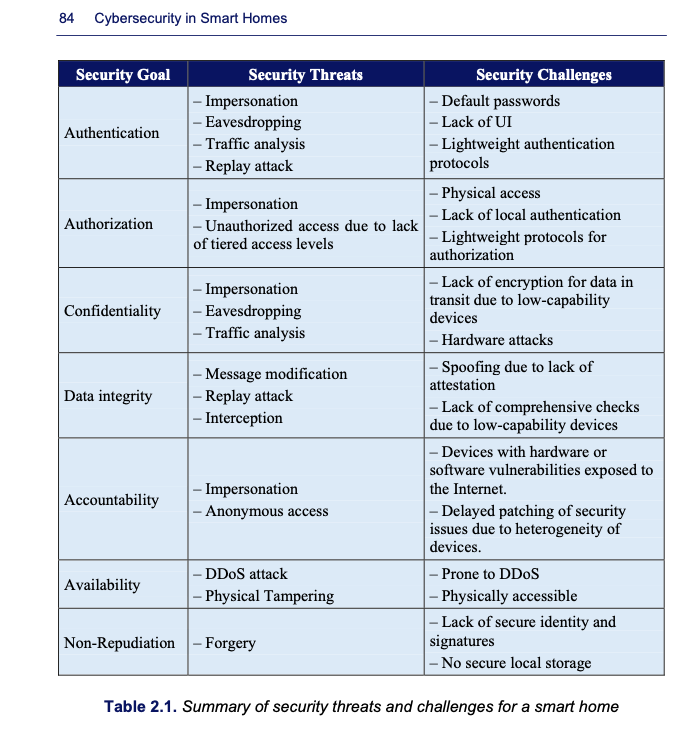
\includegraphics[scale=0.7]{resources/Table 2.1.png}

IoT devices face challenges in leveraging Internet protocols due to their low energy and limited memory capabilities. To overcome these limitations, the Internet Engineering Task Force (IETF) has developed lightweight communication protocols for different layers. Commonly used protocols include 6LoWPAN for the physical layer, RPL for routing, and CoAP for the application layer. And the three key protocols used in IoT networks are 6LoWPAN, RPL, and CoAP. 6LoWPAN enables the transmission of IPv6 over low-power wireless personal area networks. RPL is a routing protocol specifically designed for low-power and lossy networks and it is a protocol based on distance vectors and is mainly used in 6LoWPAN networks. CoAP is an application layer protocol optimized for constrained devices, offering efficient data exchange using the REST ((Representational State Transfer)) model and employing DTLS ( (Datagram Transport Layer Security) for secure communication. DTLS is based on UDP, while TLS is based on TCP since the implementation of TLS (Transport Layer Security) is complicated for constrained devices.

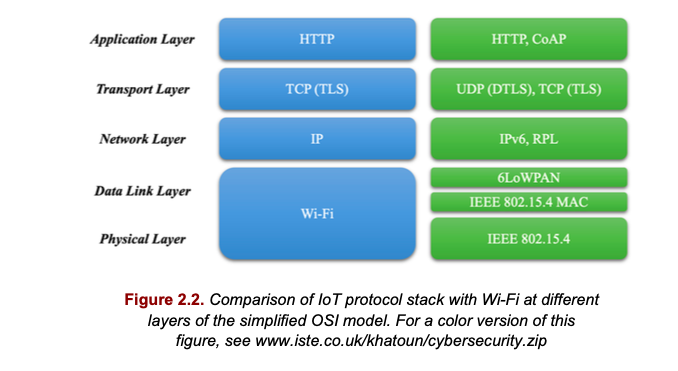
\includegraphics[scale=0.7]{resources/2.3.3.png}

Research on IoT security has led to the development of different architectures, including Cloud of Things (CoT), fog computing, edge computing, and gateway architectures. Middleware systems are commonly used for communication with IoT devices. These architectures aim to enhance security and provide solutions for complex processing, near-real-time reactions, and centralized coordination. Gateway architecture offer proxy support even without connectivity.


Here is a summarized list of some secure IoT architectures:
\begin{enumerate}
    \item SMEPP (Secure Middleware for P2P) (Benito et al. 2009): A secure middleware for peer-to-peer communication in IoT networks.
    \item FIWARE (Glikson 2011; Fazio et al. 2015): is an IoT middleware with a framework that supports a variety of plugins. Security is implemented through plugins for identity management, authorization policy, and policy enforcement points.
    \item IoT Cloud on CoAP (Kovatsch et al. 2014): is an IoT cloud architecture based on CoAP protocol that uses DTLS for security.
    \item Cloud of Things for smart home (Alohali et al. 2014): is a secure Cloud of Things architecture for smart homes where symmetric key encryption is applied to encrypt end-to-end communications.
    \item Cloud-Sensor Secure architecture (Razvi et al. 2015): has the automation of processes and data analysis done in the Cloud. The slave server manages the security of the sensors and devices on the edge.
    \item IAGW (Ding et al. 2016): An Integrated Access Gateway architecture with standard interfaces for Smart Home environments, including a security module for authentication, authorization, and encryption.
    \item Smart Home automation using WSN (Pirbhulal et al. 2017): uses Triangle Based Security Algorithm (TBSA) to ensure energy-efficient data encryption, thus providing a secure IoT-based Smart Home automation system.
    \item SH-BlockCC (Singh et al. 2019): is a secure IoT smart home architecture based on cloud computing and blockchain technology. The model utilizes the MCA (Multivariate Correlation Analysis) technique to analyze the network traffic and identify the correlation between traffic features.
\end{enumerate}

The following table summarizes the security architectures and the security goals that each promises to protect.


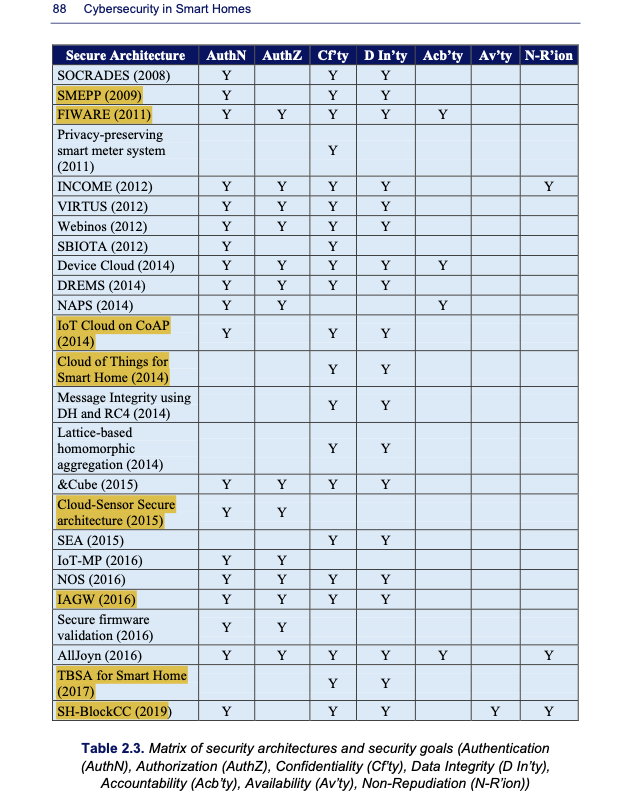
\includegraphics[scale=0.7]{resources/Table 2.3.png}

Several authentication and authorization methods exist for smart devices. These methods rely on different factors that fall into three categories:
\begin{enumerate}
    \item something a person knows (such as a password or secret code).
    \item  something a person is (such as a fingerprint or retina pattern).
    \item and something a person has (such as a smart card or digital key).
\end{enumerate}
These factors are used to establish the identity of individuals or systems in smart device authentication and authorization processes.

The authentication mechanism could be of two broad types – intra-domain (within-network authentication) and inter-domain (outside-network authentication). Intra-domain authentication could be done by any one of the above mechanisms – proof by knowledge, proof by possession, or proof by property (Mantas et al. 2011). Inter-domain authentication should ideally involve additional factors, say, a combination of proof by knowledge and proof by possession, but that is not the case many times.

The use of ID-password-based authentication has been widely adopted but has proven to be ineffective in ensuring security. Many smart home devices come with default passwords that are not changed by users, making them vulnerable to attacks. A study conducted in 2015 found that most devices lacked strong password enforcement, leaving them susceptible to breaches. Adding IoT devices to a network can compromise the overall security of the system. Guessing passwords or using weak passwords remains a common cause of security breaches. While implementing stricter password requirements can help, additional authentication factors are necessary to enhance security. Biometric factors can be used when the user is physically present, but for remote access through APIs, alternative methods must be considered.


Ferrag et al. propose a step-by-step approach for implementing an authentication protocol in an IoT system. The process includes defining the network model, choosing an authentication mechanism, considering relevant attack models, selecting appropriate countermeasures, determining when to use the authentication protocol, conducting a security analysis, and evaluating performance.


Examples of authentication mechanisms include password-based, smart-card-based, biometric, mutual, and RFID authentication. Countermeasures involve cryptographic methods, biometrics, and the fuzzy extractor technique. Formal security verification tools like ProVerif, BAN-logic, or AVISPA are used for security analysis, and performance evaluation considers factors such as communication overhead, storage cost, and computation complexity.

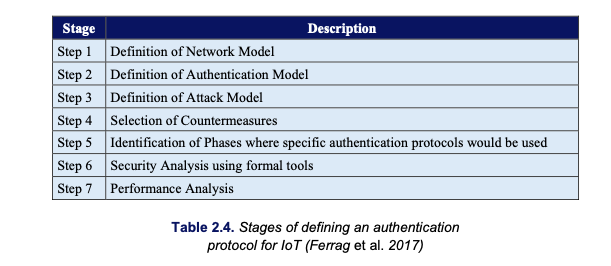
\includegraphics[scale=0.7]{resources/Table 2.4.png}

\newpage
\textbf{Mutual authentication or two-way authentication ensures that both entities involved in communication authenticate each other. It prevents unauthorized access and tampering with device states. There are different methods to implement mutual authentication: using a shared secret, public keys, or timestamps.
\begin{enumerate}
    \item Mutual authentication using a shared key: Party A and Party B securely share a key beforehand. Party A sends a message to Party B, who responds with a random challenge. Party A encrypts the challenge with the shared key and sends it back. They exchange encrypted challenges to verify authenticity.
    \item Mutual authentication using public key cryptography: Party A and Party B each have a public-private key pair. When A wants to communicate with B, A encrypts the message with B's public key or signs it with their private key. B decrypts the message or verifies the signature using their private key.
    \item Mutual authentication using timestamps: Party A sends their username and the current timestamp encrypted with a shared key to Party B. B decrypts the timestamp, increments it, encrypts the new timestamp with another shared key, and sends it back to A along with their username.
\end{enumerate}
These methods ensure that both parties authenticate each other before exchanging messages, adding an extra layer of security to the communication process.}

The following table summarizes different types of authentications grouped by authentication factors and types.

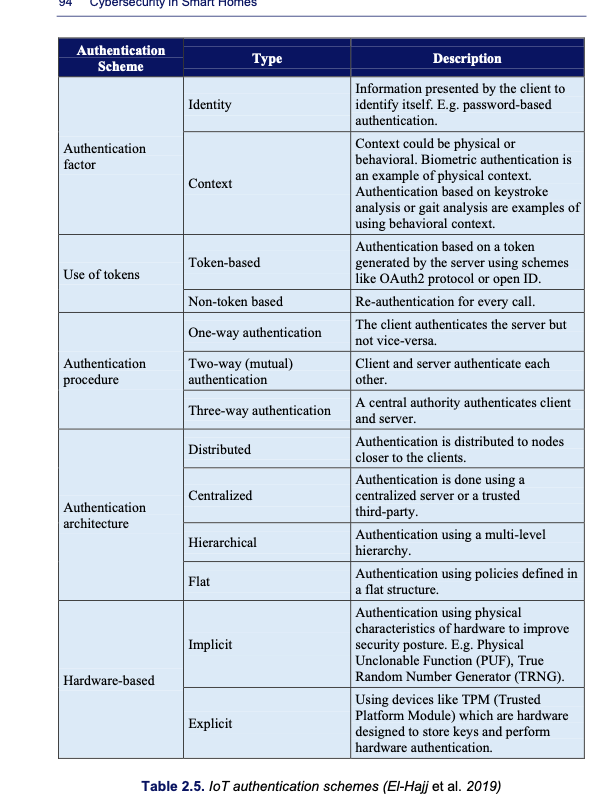
\includegraphics[scale=0.7]{resources/Table 2.5.png}

\newpage
SSL (Secure Sockets Layer) was the basis for the TLS (Transport Layer Security) standard (Dierks and Rescorla 2006) defined by the IETF (Internet Engineering Task Force).

\textbf{TLS (Transport Layer Security) is a protocol that provides security and reliability for communication between applications over the internet. It sits between the application layer (e.g., HTTP) and the transport layer (e.g., TCP) and ensures the availability of TCP features like reliability and flow control.}

\textbf{TLS offers three main properties for securing applications:
\begin{enumerate}
    \item Server authentication: The client can verify the identity of the server using public-key cryptography.
    \item Secure and reliable connection: The communication between the client and server is encrypted using symmetric cryptography, ensuring confidentiality, and each message includes a check to ensure message integrity.
    \item Client authentication: The server can authenticate the client using public-key cryptography.
\end{enumerate}
In web applications, TLS is commonly used to authenticate the server and establish a secure connection. In mutual authentication, both the client and server authenticate each other using digital certificates to prove their identities before the actual communication takes place.}


\textbf{TLS 1.3}
TLS 1.3 was introduced to secure connections with low-capability IoT devices. It reduces the number of round trips required for the handshake, cutting encryption latency in half. TLS 1.3 uses key agreement algorithms and KeyShares to complete the handshake in fewer round trips. It also introduces the ServerConfiguration packet, which enables remembering previous connections, further reducing the round trips. Lightweight IoT devices use ECC (elliptic curve cryptography), which offers the same security level as RSA but with smaller keys.

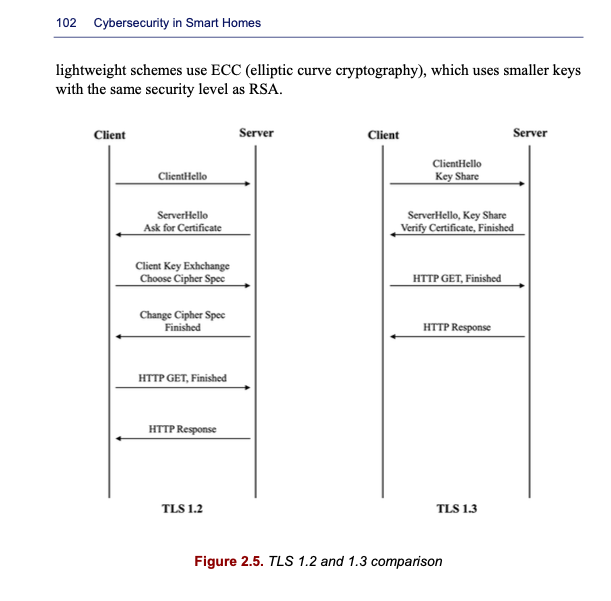
\includegraphics[scale = 0.7]{resources/Figure 2.5.png}


\textbf{X.509 certificate}

X.509 is a standard for public-key certificates used in mutual authentication. It includes a public key and an identity, and can be signed by a Certificate Authority (CA) or self-signed. The mutual authentication process involves different certificates:
\begin{enumerate}
    \item Root CA certificate: A self-signed certificate that identifies the CA that signed a client's certificate. In IoT setups, administrators deploy the root CA certificate or chain to edge servers.
    \item Server SSL certificate: Deployed on the server and sent to the client during TLS handshake.
    \item Client SSL certificate: Deployed on the client and sent to the server during mutual authentication.
\end{enumerate}

X.509 certificates are commonly used in industrial IoT trust implementations. Device manufacturers certify and sign the keys assigned to the devices.

An X.509 certificate contains various fields such as version, serial number, issuer's signature, issuer, validity period, subject, subject public-key info, unique identifiers, extensions, and the CA's digital signature.

While X.509 certificates provide strong identity and access control, they require devices to have sufficient computational power, which may not be available in IoT devices. However, this is being addressed by newer devices with increased computational power and the development of standards for devices with computational constraints, such as the IEEE 1609.2 certificate format that uses elliptic curve cryptographic algorithms.

The sequence of certificate exchanges and establishment of an encrypted channel for communication using mutual certificate-based authentication is depicted in Figure 2.3.

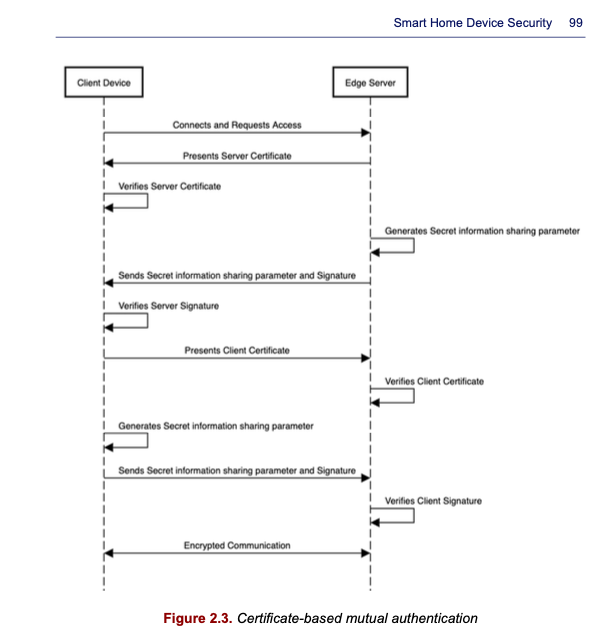
\includegraphics[scale=0.7]{resources/Figure 2.3.png}

 \newpage
\textbf{Mutual authentication in smart home systems}

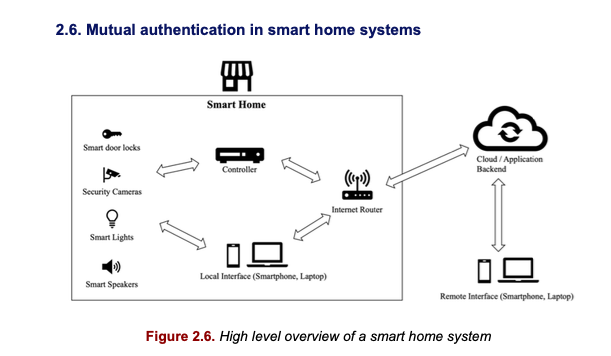
\includegraphics[scale=0.7]{resources/Figure 2.6.png}

Figure 2.6 illustrates a smart home network with various communication channels between devices. Multiple gateways may exist, connecting different devices based on their manufacturers or functionalities. A smartphone can connect to these devices through the gateway, simplifying the network structure. The gateway architecture is commonly used as it facilitates translation between IoT standards, maintains a consistent security scheme, and enables device connectivity to the Internet.

During the initiation phase, mutual authentication takes place. When a new device is added to the system, it undergoes authentication during the initial pairing process. A certificate is created and verified using the manufacturer's private key. The authentication module determines whether the new connection is allowed or not. The user registers with a trusted authority, while the devices are already registered. The gateway serves as the central node responsible for network control, device interoperability, and secure management. After successful registration, the trusted authority stores the authentication information in the smartphone and gateway memory.

Mutual authentication occurs between the user and the gateway, between the gateway and the smart devices, and between the user and the smart devices. They establish a secret session key to protect exchanged messages. A symmetric session key, such as AES-CBC, is used for future secure communications.


Device onboarding consists of two main steps:

\begin{enumerate}
    \item device provisioning: During device provisioning, the device registers itself to the IoT platform when it first connects online. The device's unique certificate is created by the manufacturer using a registered root CA and stored in the device firmware. When the device connects to the platform, the certificate is validated against the platform's root CA, allowing the device to connect multiple times in the future.
    \item device linking: The next step is device onboarding, where a user identity is linked to the device. The user obtains an activation code from the device, which can be found on the device itself, its packaging, or provided through the phone. The user submits this code to the platform, which associates the user with the device and sends this information to the gateway or device for further authentication and access control.
\end{enumerate}

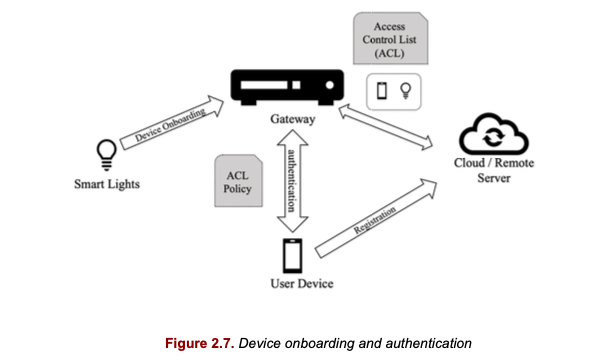
\includegraphics[scale=0.7]{resources/Figure 2.7.png}

\textbf{The flow of user authentication and authorization in a smart home network is as follows:}
\begin{enumerate}
    \item Device Authentication: When a device wants to access a sensor through the gateway, it goes through the authentication process. This involves exchanging keys and validating credentials with the gateway or remote server.
    \item Session Initialization: Once the authentication is successful, the platform generates a session ID to keep track of all the actions performed during that session. The session ID helps in maintaining the continuity of the user's interactions.
    \item Authorization Check: When the user initiates any action, such as controlling a device or accessing sensor data, the gateway checks the Access Control Lists (ACLs). ACLs contain rules and permissions that determine whether the user is authorized to perform the requested action.
\end{enumerate}
By going through the authentication process and passing the authorization checks, the user can securely interact with the smart home network and perform authorized actions based on their assigned privileges.

\textbf{To summarize, the key challenges and open research issues in the context of smart home networks are as follows:}

\begin{enumerate}
    \item Smartness in routers and modems: Research is needed to develop universal routers that can perform the functions of specific company hubs, enhancing security and reducing complexity for users.
    \item Auto configuration support: Secure auto-configuration mechanisms should be developed to simplify the installation and management of smart home devices, reducing the risk of security vulnerabilities.
    \item Standardization of device upgrades: Research is needed to address the challenges related to providing security patches and upgrades for IoT devices, ensuring a more consistent and secure environment.
    \item Built-in security and privacy goals during design: Guidelines should be established for manufacturers to incorporate security measures into smart devices from the design phase, focusing on mitigating risks, protecting confidentiality and privacy, and ensuring system availability and resilience.
    \item Regulation in the industry: Standardization and regulation are necessary to enhance transparency and privacy protection for consumers. Ideas such as adopting "nutrition label" concepts for smart devices can promote awareness and accountability among manufacturers.
    \item Improved awareness and knowledge: Efforts should be made to educate and raise awareness among the general public about the security and privacy aspects of smart home devices. Research on the correlation between consumer tech-savviness and the reduction of cyberattacks can inform policymakers and industry stakeholders.
\end{enumerate}
Addressing these challenges and conducting research in these areas will contribute to the development of more secure, user-friendly, and privacy-preserving smart home networks.

\newpage
\subsubsection{Chapter 4 By Zohreh Asadi:}

IoT smart home automation is a rapidly growing global trend, but it also presents numerous concerns and challenges. The utilization of data to observe, manage, and transmit information between devices over the Internet enables remote actions based on specific conditions. However, effectively managing and securing IoT smart home devices is a complex task that requires careful attention. Monitoring, energy management, and data protection necessitate efficient control and management strategies. As the deployment of smart home IoT infrastructure continues to increase, network security becomes a major area of concern. This chapter explores the challenges and implications of IoT network security for smart homes.

IoT-based smart home security involves the use of devices and sensors to remotely control and monitor services for customers. Initially introduced in the 21st century, smart home tools and technologies empower users to control their home devices through apps or networked devices. Ensuring security in IoT-based smart homes is of paramount importance due to the vulnerability of various devices to attacks. Lightweight security apps and technologies can help address these challenges effectively.

Wireless network solutions like Bluetooth play a significant role in supporting IoT-based home systems. With the rise in popularity of smart homes, security has become a top concern. Implementing access monitoring and control systems, along with robust communication procedures, can significantly enhance smart home security. The protection of confidential information, such as addresses and network-related data, remains a critical aspect; however, limited options are available in this regard.

The confidentiality and security associated with IoT-related information processing and threats are continuously being analyzed. Government associations are increasingly involved in developing IoT-based security and interoperability standards. Regulations, standards, guidelines, policies, and procedures all play crucial roles in enhancing security and mitigating risks in smart homes.

While standards are not yet mandatory in IoT-based smart home systems, they play a vital role in the development of innovative tools and techniques. Application-related techniques such as facial recognition, fingerprint scanning, and password protection have demonstrated improvements in security. The convergence of machine learning, wireless communications, embedded systems, and real-time analytics has opened up new possibilities for IoT applications.

The text delves into various prevailing standards and initiatives in the field of smart home security, particularly concerning the Internet of Things (IoT). It emphasizes the increasing adoption of IoT in smart homes and the subsequent rise in IoT security concerns. The European smart home security market is projected to reach 7.95 billion USD by 2024.

To address the challenges posed by IoT security, several home security standards have been developed to ensure interoperability among a wide range of associated products and services. The Open Connectivity Foundation (OCF) has played a significant role in promoting interoperability by integrating the AllJoyn and IoTivity open-source frameworks. These frameworks facilitate seamless communication and interoperability within the IoT ecosystem.

Another notable organization, the Zigbee Alliance, focuses on interoperability in smart home systems. Zigbee technology is widely implemented by global service installers, suppliers, and dealers, enabling interoperability between different products irrespective of the manufacturer.

The Bluetooth Special Interest Group (SIG) promotes Bluetooth Low Energy, offering a power-friendly wireless technology for smart home devices that allows direct control from portable devices such as smartphones or tablets.

The text also mentions other noteworthy initiatives, including IFTTT (If This Then That), which enables devices to communicate and automate actions; open APIs provided by companies like Samsung and Apple, encouraging device integration; Thread, a low-power wireless network standard for smart home security; Constrained Application Protocol (CoAP), a communication protocol for resource-restrained IoT devices; and Datagram Transport Layer Security (DTLS), providing secure communication over untrustworthy datagram protocols.

Collectively, these standards and initiatives aim to enhance security, interoperability, and ease of use in the rapidly growing field of smart home technology.

IoT applications encompass various areas, including remote monitoring and control of smart home devices, energy consumption management, and security systems. Key components such as Android applications, web server databases, control units, sensors, cameras, and motion sensors are essential for controlling and monitoring smart homes. Additionally, relay modules, gas and smoke sensors, light sensors, alarms, and GSM modules enhance the functionality and security of smart homes.

In conclusion, while IoT-based smart home automation brings convenience and efficiency, it also presents security challenges. Implementing robust security measures, adhering to regulations and standards, and adopting reliable technologies are crucial for ensuring the safety of smart homes and protecting user data.

The security of IoT networks in smart homes remains a significant concern, with various strategies being developed to combat network attacks. These attacks often employ customized or new techniques that bypass detection mechanisms, posing an ongoing problem. Network security in IoT is established at different levels, and customers expect IoT devices to have built-in security measures.

The complexity of network security challenges has increased as the range of devices expands beyond computers to include operating systems like MacOS, Linux, and Windows, as well as wireless protocols such as BLE, Bluetooth, NFC, ZigBee, Wi-Fi, LoRaWan, and Thread. The Internet Engineering Task Force (IETF) has made efforts to establish lightweight communication protocols, including IPv6 over Low Power Wireless Personal Area Networks (6LoWPAN), IPv6 Routing Protocol for Low power and Lossy Networks (RPL), and the Constrained Application Protocol (CoAP).

At the network level, security measures are implemented to protect IoT devices. Access control procedures safeguard the devices, and security management providers (SMPs) connect with internet service providers (ISPs) and home routers to configure and control security. SMPs offer customizable interfaces, allowing customers to manage security settings. ISPs and router vendors can reduce management overhead by using cloud-based controls and automated network APIs.

Embedded devices play a crucial role in securing IoT-based smart homes, encompassing a wide range of appliances and systems. Virtual or cyber security measures are essential to protect IoT systems from hackers. Customers also play a role in enhancing security beyond the ISP or router vendor. The network controller of the ISP uses the Floodlight OpenFlow controller, while SMPs utilize security composers or Ruby-on-Rails to handle security procedures. Web-based apps provide customers with front-end support for modifying services and accessing security settings.

Service providers and supporting devices like Nest smoke alarms and Philips Hue lightbulbs contribute to the overall security ecosystem. Mobile apps can enable secure access to IoT devices, and some suppliers offer IoT security as a service by actively monitoring and controlling network-level functions.

In conclusion, ensuring network security in IoT environments is crucial for smart homes. Multiple stakeholders, including customers, ISPs, router vendors, SMPs, and security service providers, must collaborate to implement robust security measures at various network levels to protect IoT devices

\newpage
\subsection{Quelle: \cite{s23031252}}
\subsubsection{By Zohreh Asadi}

The Internet of Things (IoT) is a global movement that brings together interconnected smart devices, enabling them to exchange information with minimal human intervention. This revolutionary technology is advancing rapidly, and by 2025, an estimated 27 billion devices are expected to be connected. While IoT offers numerous smart applications that enhance our quality of life, the sheer volume of data generated raises concerns about user privacy. By the end of 2022, it is predicted that 15 billion smart devices will be connected, further intensifying the privacy challenge. Users struggle to maintain control over the data shared by their devices, leading to the adoption of privacy regulations such as the EU General Data Protection Regulation (GDPR) in 2018, which aims to empower users with control over their personal data.

To address privacy concerns in IoT environments, this paper presents a comprehensive survey of machine learning (ML) techniques relevant to privacy protection. The objective is to identify and classify privacy threats in IoT, explore the challenges associated with applying ML to privacy protection, review existing research on ML techniques for privacy protection in IoT, and propose future directions for further study. The survey is divided into sections that cover the identification and classification of privacy threats, the review of ML-based solutions, and a concluding section that discusses challenges and future directions for privacy preservation in IoT systems.

Previous research has primarily focused on addressing cybersecurity threats in IoT, with limited attention given to privacy-focused surveys and specific solutions. Some surveys have analyzed ML-based cybersecurity solutions but have provided minimal content on privacy. For instance, Al-Garadi et al. reviewed ML-based IoT solutions, examining vulnerabilities and attack surfaces. Similarly, Hussain et al. reviewed ML-based solutions for IoT cyberattacks in the areas of network, malware, and privacy. Waheed et al. provided an overview of ML-based cybersecurity solutions, including techniques like Stochastic Gradient Descent (SGD), Logistic Regression (LR), Oblivious Evaluation of Multivariate Polynomial (OMPE), Support Vector Machines (SVM), and Naive Bayes (NB). Khan et al. focused on ML-based cybersecurity solutions for 5G networks and privacy issues related to the usage of user private data by service providers.

Other works have specifically reviewed deep learning (DL)-based solutions for privacy and cybersecurity. Dixit and Silakari reviewed existing cybersecurity threats and DL-based solutions for privacy. Rodriguez et al. surveyed DL-based solutions for various types of cyberattacks in mobile networks, categorizing them into collaborative DL, differential privacy, and training on encrypted data. Gosselin et al. reviewed privacy and security issues related to Federated Learning (FL) and highlighted inference-based attacks as the most critical. Tanuwidjaja et al. and Boulemtafes et al. provided reviews of privacy preservation in DL solutions. The primary challenge in privacy-preserving ML techniques is finding the right balance between accuracy and complexity.

Zheng et al. conducted a taxonomy of existing privacy-preserving ML approaches and classified them into three main groups: privacy-preserving model training or learning, privacy-preserving inference or analysis, and release of a privacy-preserving model. Homomorphic encryption is the most commonly used concept for privacy-preserving model learning and inference, while differential privacy is frequently used for releasing privacy-preserving models. Liu et al. and Ma et al. focused on improving the homomorphic encryption scheme to prevent privacy leakage in FL. They proposed a two-phase encryption scheme that combines the Paillier cryptosystem with a secret sharing mechanism. The scheme achieves privacy preservation in FL while maintaining high accuracy in DL tasks.

Another approach for privacy-preserving ML in IoT is the use of secure multi-party computation (SMC) techniques. SMC allows multiple parties to jointly compute a function on their private inputs without revealing the inputs to each other.



\newpage

    \nocite{*}
    \bibliography{src/referencias}


\end{document}
